The core components of Killerbeez can be split into two logical categories:
those which are related to orchestration, and those related to feeding data
to the target\footnote{Software under test is referred to a the ``target.''}
program and collecting results.  The former refers to decisions such as what
inputs to use as seed data,\footnote{Initial inputs which will be modified
are referred to as ``seeds.''} which mutation algorithms to use, how to minimize
the input corpus and other decisions which are best left to a central
controller.  The latter category contains actions such as launching the target,
feeding the target input data, tracking code coverage, determining when the target is
done processing the input and reporting whether the target crashed, froze due
to something like an infinite loop, or executed new portions of code.

\subsection{Orchestration}
All of the orchestration tasks are handled by the manger running on a central
server.  It decides what mutators will be used on each target,
handles minimizing interesting inputs, determines if crashes
and hangs are unique, and identifies inputs that can be dropped because the code they
reach is already covered by other inputs. A \BOINC{} server is used to transmit
the work to worker nodes and receive results.  All of this is depicted in
Figure \ref{fig:Killerbeez-server}.

\begin{figure*}[htb]
\centering
\includegraphics[width=6in]{KILLERBEEZ_Server_Architecture.png}
\caption{Killerbeez Server Architecture}
\label{fig:Killerbeez-server}
\end{figure*}

\subsubsection{Manager} \label{Manager Overview}
The manager combines all of the server side components.  It is
primarily a bookkeeper to track which targets are available for fuzzing,
queue jobs\footnote{``jobs'' is a \BOINC{} term here, referring to a unit of work.} to be served to \BOINC{} clients, process the results to
determine if code paths are unique, and interface with external components.

Because the manager is not responsible for running the target application, it
does not need to run on the same platform as the target.  It can happily run on Linux and
serve work to be executed by Windows or macOS machines and collect the
results.

The manager will enable future enhancements to be made by taking advantage of
external tools, such as
using a test case generator to produce new seed data. Another planned integration
is to use Driller\cite{driller} to generate program inputs which reach
code which has not yet been reached by mutation. These integrations are made
possible by providing a \REST{} \API{} to the manager component, which allows clients
to access and configure seed data, fuzzing targets, and low-level metadata
produced during fuzzing.

The \API{} is also used for some of the manager's built-in functionality. The
campaign manager, which plans out jobs to be
executed, consists of pluggable modules to choose the job's type, inputs, and
parameters. The \API{} is used by these modules to gather the data they need,
and then submit fuzzing jobs. The corpus
minimization uses this \REST{} interface to obtain
execution traces and modify the working set of seed values. This allows components to be
less coupled with the internals of the manager, enabling them to run as
standalone processes. Figure
\ref{fig:Killerbeez-integrations} shows how these tools can interface with the
manager via the \REST{} \API{}.

The manager can decide how long each job takes by specifying things like the
number of fuzz iterations, so it should be able to scale up to a very large number
of clients by ensuring each job takes a long time.  This will allow a substantial amount of
work to get done with a minimal amount of coordination and network overhead.
However, if the manager becomes a bottleneck, multiple
manager servers could be set up and the \REST{} interface used to share
information between them.

\begin{figure*}[htb]
\centering
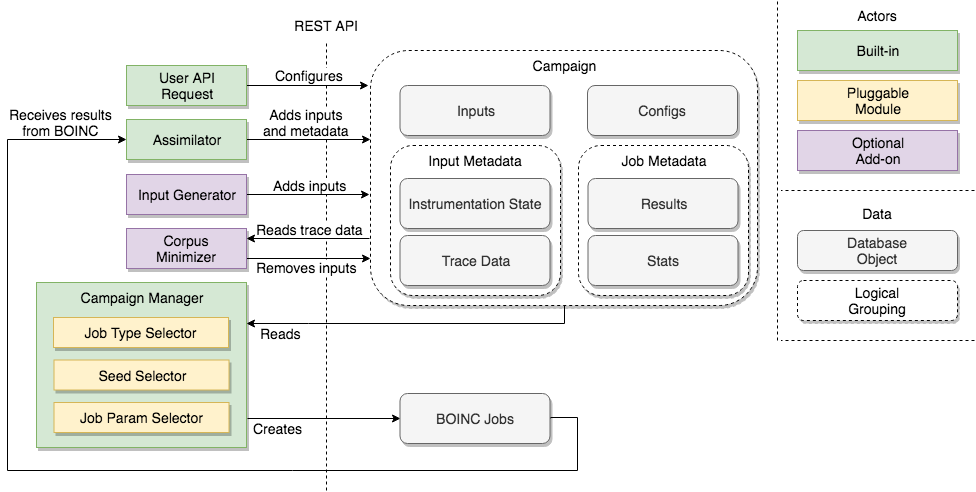
\includegraphics[width=6in]{KILLERBEEZ_Integrations.png}
\caption{Killerbeez Integration with External Tools}
\label{fig:Killerbeez-integrations}
\end{figure*}


Killerbeez also introduces the idea of obtaining detailed information about
execution for each input which has a unique code path.  This is typically
not done by other fuzzers, as obtaining a full trace is much more overhead than
the lightweight instrumentation that \AFL{} or Honggfuzz use. During
normal fuzzing, Killerbeez will generally use lightweight methods of tracking
execution. However, having a full trace is useful when minimizing the seed corpus
and determining which seeds should be weighted more heavily. This concept has
been encapsulated in the tracer module.
Each time an input
is found which hits a new code path, a tracer job can be added via the manager.
This job will be executed by a \BOINC{} client, just like any other fuzzing job.
The results will include full trace data, which will be stored in the manager's
database.  More information about the tracer can be found in section
\ref{Tracer}.

\subsubsection{Preparation}  \label{Preparation Overview}
There is a preparation phase of fuzzing workflows which is often overlooked or
dismissed, that includes setting up the target software and deciding specific
fuzzing parameters. This occurs before any real fuzzing begins and includes
things such as compiling the target, possibly with a specific compiler or
compiler flags, determining what options should be enabled in the target
software, deciding which portions of the code should be tracked for code
coverage, and specifying how to deal with non-deterministic code.

The compilation step is driven by the type of instrumentation chosen,
which is typically just a matter of choosing the option with the lowest
performance penalty. Instrumentation does not need to be added at compile
time, but it is added here when possible, as it reduces the overhead at runtime.
What options to enable in the target software is target specific and
subjective.  It depends on the higher level goals.  If the goal is to find a
vulnerability with wide applicability, choose default options. If it is to test
out a specific feature, disable everything except that option. If it is just to
find any bug in any configuration, enable everything.  While these are
important questions, the most interesting decision is what to track in terms of
code coverage, and how to deal with non-deterministic code.

The solution \AFL{} uses is to require the user to manually determine which code
in the target to instrument. \AFL{} requires the user compile the target library
or executable with a special instrumenting compiler. Alternatively, \AFL{} can
use a modified version of QEMU while fuzzing to instrument all of the libraries
used by a target at run-time.  As expected, instrumenting all of the libraries
has a higher overhead than only instrumenting a few specific modules. Killerbeez
improves on this by including a tool
called the ``Picker'' which automatically determines which libraries should be
instrumented.  The algorithm for doing so is described in section \ref{Picker}.

One important detail is that the picker can not operate effectively when the
target does not have deterministic execution.  If feeding the same file into
the application multiple times results in different code being executed, this
is a problem, not only for the Picker, but also for code coverage in general.
\AFL{} does not deal with this problem directly, but it does alert the user to
the fact that the target is non-deterministic. The user can then do things like
hijack calls to functions such as \texttt{srand()} which intentionally introduces
randomness. This is often done for applications which employ cryptography for
initialization vectors and nonces. Under command line Linux applications, this
works fairly well.  On GUI applications in Windows, it does not work as well.
There are system calls in Windows which occasionally fail for no apparent reason. This
should not be a problem for the target software, as it should be checking the return code to
detect and handle this appropriately.  However, when this happens it has the
side effect of making the fuzzer misinterpret the new code coverage to think an input was interesting when it was
not.  The details of how non-determinism is handled in Killerbeez are also described in
section \ref{Picker}.

\subsection{Execution}
Execution is handled by the client fuzzer program, which is aptly named ``fuzzer.''
This can be run manually from the command line, however it is typically run by
the manager, via a \BOINC{} client.  In either case, the fuzzer is responsible
for running the target, feeding it input data, tracking code
coverage, detecting crashes, and dealing with user interaction such as dialog
boxes.

\begin{figure*}[htb]
\centering
\includegraphics[width=6in]{killerbeez-high-level-block-diagrams.png}
\caption{Killerbeez Fuzzer Overview}
\label{fig:Killerbeez-fuzzer-overview}
\end{figure*}

The fuzzer consists of glue code that combines together various
modules, which is where all the interesting things occur. The purpose of
the Driver, Mutator and Instrumentation modules used in the fuzzer are covered in sections
\ref{Driver Overview}, \ref{Mutator Overview}, and
\ref{Instrumentation Overview}, respectively.  The relationships between these components are depicted in Figure \ref{fig:Killerbeez-fuzzer-overview}. The modules which currently
exist and how they work are covered in the \nameref{Implementation}
section.

The same code base is used on Windows, Linux and macOS to enable as much code
re-use as possible.  Most of the mutators are shared among all platforms.
Some of the instrumentation and driver\footnote{
``driver'' refers to driver modules, not operating system drivers.}
modules contain platform specific and sometimes target specific code.

\subsubsection{Driver} \label{Driver Overview}
Killerbeez offers drivers, which are target-specific wrappers that abstract
away the concept of loading data into a target and enable finer
definition of the failure modes of a particular piece of software. While
typical fuzzers look for crashes and hangs, specifically-written drivers can
have more context about a given fuzz target.  Better understanding of the fuzz
target's behavior means that Killerbeez can make better-informed decisions
about the status of a target after a particular input, and it can terminate or
classify the result of a particular input more quickly than waiting for a
timeout.

First, the driver module is responsible for feeding inputs to a target.  This
is a departure from most fuzzers, which only work for one type of input.  In
the case of AFL, the input is a file or stdin (which is also a file under
UNIX).  Syzkaller\cite{syzkaller}, on the other hand, uses only system calls.
Each tool then has to implement their own mutation algorithms, code coverage,
results collection and so forth. Drivers enable Killerbeez to reuse all of
these components and select how to interact with the target by simply selecting
the appropriate driver.  Abstracting this away allows for more exotic use
cases, such as fuzzing \IOCTLs{}, network servers, network clients, \IPC{} such as
Mach Messages, XPC, Distributed Objects, \COM{}, and others, all with minimal
effort.

The second thing drivers are responsible for is dealing with any target
specific issues, such as handling GUI interactions.  For example, if a PDF file
with a malformed header is given to a PDF reader application, it typically will
pop up a dialog box indicating that the file is corrupt. Fuzzers such as
Honggfuzz or WinAFL would wait until a timeout expires.\footnote{WinAFL can
exit at the end of a function, but dialog boxes tend to prevent that function
from returning in practice.} This results in all executions which hit this code
path to appear as a hung process.  In Killerbeez, a driver could be written for
the specific PDF reader which monitors the application for dialog boxes,
detects when dialog boxes appear, analyzes the text of the dialog box and
determines that the status is a clean exit rather than a hang.  This would allow
the fuzzer to move on to the next input more quickly, as it would know the
input is done being processed and would not need to wait the full timeout
period.  It also helps discern between a hang, which may indicate a Denial of
Service vulnerability such as an infinite loop, and an error which is handled
in the expected manner. For another example, see the Windows Media Player
driver in section \ref{Driver}.

Many of the drivers will work on many fuzzing targets in a particular category.
Targets which accept input from the network, are handled by the Network Server
driver module, programs which open a file are generally handled by the file
driver and so forth.  Other drivers can be written to handle things which are
specific to particular pieces of software.  Some targets will handle opening files
differently if opened via double clicking an icon as compared to using the open
option from the file menu. Other examples include error message analysis to
determine if the system should move on to the next input, or if it should click
``OK'' and continue (e.g. in the event of a warning message).

\subsubsection{Mutator} \label{Mutator Overview}
Killerbeez also implements ``mutators,'' which are abstractions on modifying
program input. They decide where to modify bytes in the input data, and how
to modify them.

Killerbeez uses a selection of user-selectable mutators. Parameters are passed
to the mutator module via the driver, which control the operation of the
mutator. For example, the bit flip mutator flips a parametrized number of bits
throughout the entire input, one at a time.

Modular mutators also enable trivial combination of different approaches. Using
the multipart mutator, different mutators can be applied to different parts of
the input. This is required for efficiently fuzzing network protocols, as it is
often desirable to not mutate the initial packets as they may include a handshake or
authentication.  Any mutation to this section would prevent the majority of code from being
executed, as the target software would execute an error path instead. It can
also be used to ensure that the first few bytes in a file are not modified so
the file will still be recognized as being the correct file type.


\subsubsection{Instrumentation} \label{Instrumentation Overview}
Instrumentation modules are responsible for tracking program execution and
determining if an input has caused the target program to execute new code. How it does this,
and what level of granularity is used, are questions left to the module author.
There is an \IPT{} instrumentation module which is very high resolution.
If a loop somewhere in the target is executed 178 times instead of 177
times, it will detect this as a new code path, as the state explored is
different than what was seen before.  The \AFL{} instrumentation module, on the
other hand, would not consider this to be an input which causes the execution of new code.
The \AFL{} instrumentation module uses a bucketing system that groups executions of the same
code and considers anything which executes a portion of code 128-255 times to
be equivalent.

Sometimes instrumentation modules need to interface with kernel drivers, which are
implemented differently on different operating systems. For instance, the \IPT{}
instrumentation module uses the perf subsystem on Linux, which is not available
on macOS or Windows. Other instrumentation technologies, such as Intel's
Pin,\cite{pin} have a very similar interface across different operating
systems, which means more of the code in the instrumentation module can be
re-used, simply using \#ifdef directives if there are portions which are
specific to a particular operating system.
